% !TEX root = main.tex

%%%%%%%%%%%%%%%%%%%%%%%%%%%%%%%%%%%%%%%%%%%%%%%%%%%%%%%%%%%%%%%%%%%%%%%%%%%%%%%%%%%%%%%%%%%%%%%%
\section{演習課題}
%%%%%%%%%%%%%%%%%%%%%%%%%%%%%%%%%%%%%%%%%%%%%%%%%%%%%%%%%%%%%%%%%%%%%%%%%%%%%%%%%%%%%%%%%%%%%%%%

\subsection{理想コイルとそうでないコイルの比較}

\begin{figure}[H]
    \begin{center}
        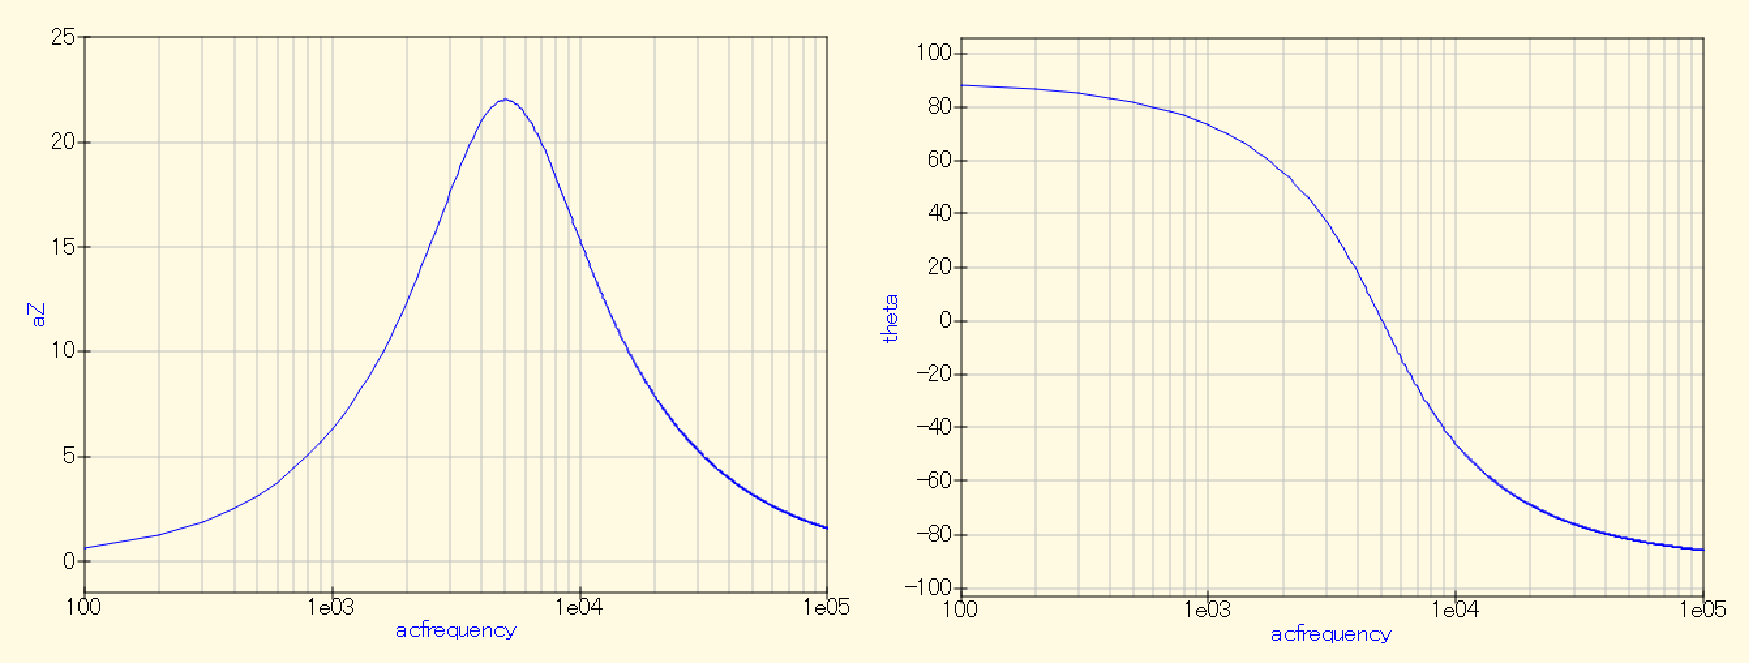
\includegraphics[scale=0.5]{ideal.pdf}
        \caption{理想コイルにおけるインピーダンス周波数特性およびインピーダンス偏角の周波数特性}
    \end{center}
\end{figure}

\begin{figure}[H]
    \begin{center}
        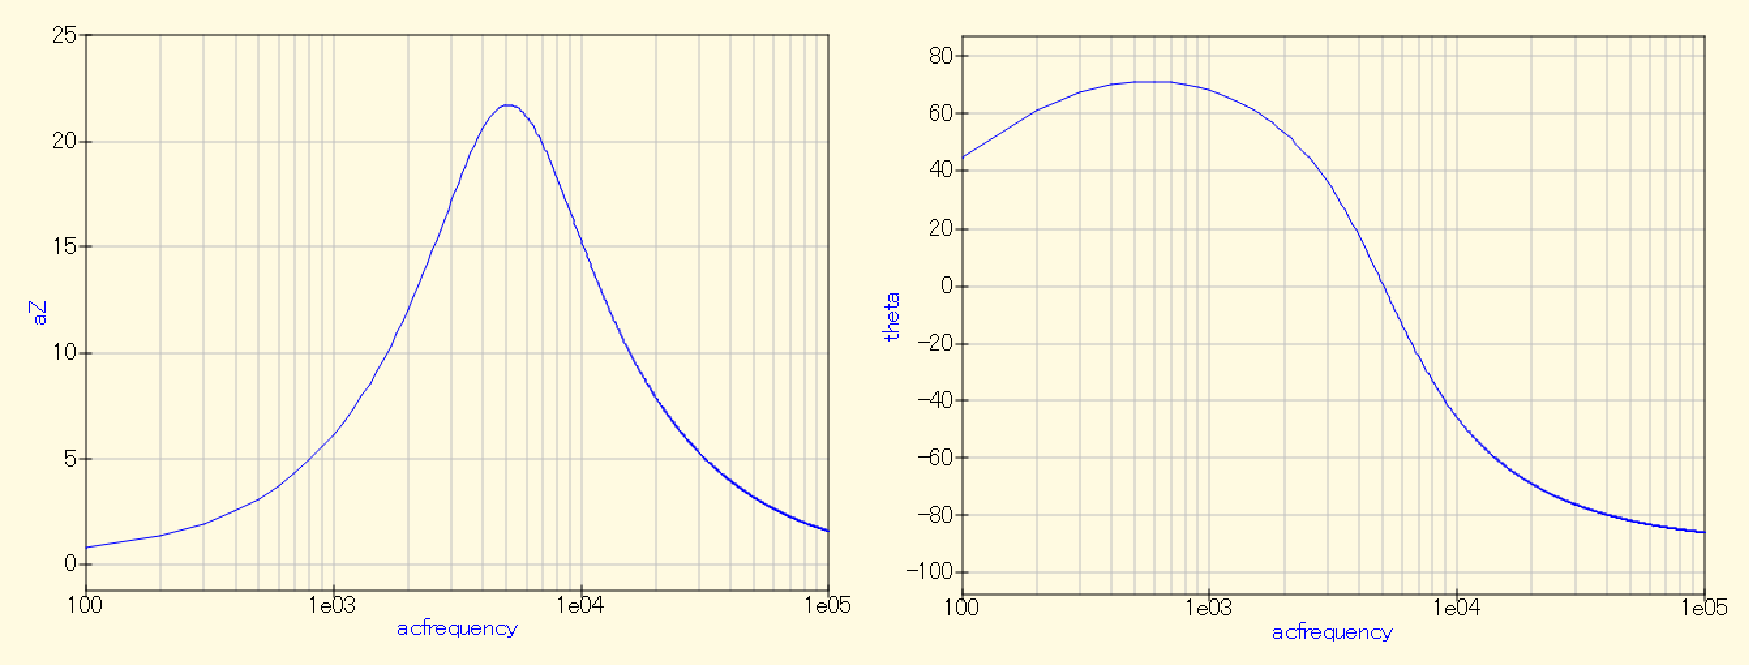
\includegraphics[scale=0.5]{not_ideal.pdf}
        \caption{理想でないコイルにおけるインピーダンス周波数特性およびインピーダンス偏角の周波数特性}
    \end{center}
\end{figure}